\documentclass[pstricks,border=11pt]{article}

\hfuzz=0.64pt
\usepackage[utf8]{inputenc}

\usepackage{amsmath} % for the equation* environment
\usepackage{tabularx}
\usepackage{multirow} % Required for multirows
\usepackage{booktabs} % For prettier tables
\usepackage{siunitx} % Required for alignment
\usepackage{pgfplots}
\usepackage{pst-plot}
\usepackage{hyperref}
\pgfplotsset{compat = newest}
\sisetup{
  round-mode          = places, % Rounds numbers
  round-precision     = 2, % to 2 places
}
\title{Sinusoidal Functions Menu Task 2}
\author{Tiffany Pham}
\date{18 November 2022}

\begin{document}

\maketitle

\section{Introduction}
Build as \textit{few} sinusoidal functions as possible to satisfy each constraint at least once.
\vspace{5mm}
\begin{center}
Include a sketch of each graph to make your thinking visual.
\end{center}

\begin{table}[!ht]
\begin{tabular}{|l|p{2in}|l|p{2in}|} 
\hline
A. & Never touches the x-axis                                & B. & Has a positive y-intercept                \\ 
\hline
C. & The amplitude is greater than the vertical displacement & D. & Has a negative "\textit{a}" value         \\ 
\hline
E. & Has exactly 1 zero on the interval [0,4]                & F. & Has a non-zero horizontal shift           \\ 
\hline
G. & Has a period length greater than 2$\pi$                     & H. & The range includes negative and positive  \\
\hline
\end{tabular}
\end{table}
\begin{center}
    \textit{Which constraints pair nicely?}
    
    \textit{Which constraints cannot be paired?}
    
    \textit{Is it possible to solve in 2, 3, or 4 functions?}
\end{center}

A, B, D, and F pair nicely, and C, E, G, and H pair nicely. The ones you can't pair are A and H because for the range to be negative and positive y-values, it has to touch the x-axis/ go through the x-axis. You also can't pair A and E because it has to touch the x-axis to have 1 zero on the interval.

I built two functions that fit all of the constraints. One function for A, B, D, F and another for C, E, G, H. Since I've built two functions, I think the least functions that this problem can have is two because both of my functions have satisfied all of the constraints.

\vspace{5mm}
\section{Functions}
Describe how and why you built each function. Be sure to identify which functions satisfy which constraints.

\hfill \break
Basic Equation
\begin{displaymath}
    y=a\sin(bx-c)+d
\end{displaymath}

\vspace{10mm} %5mm vertical space
\hfill \break
Function 1
\hfill \break
Satisfies: A, B, D, F
\begin{displaymath}
    y=-2\sin(0.5x-1)+3
\end{displaymath}

\vspace{5mm}
\begin{center}
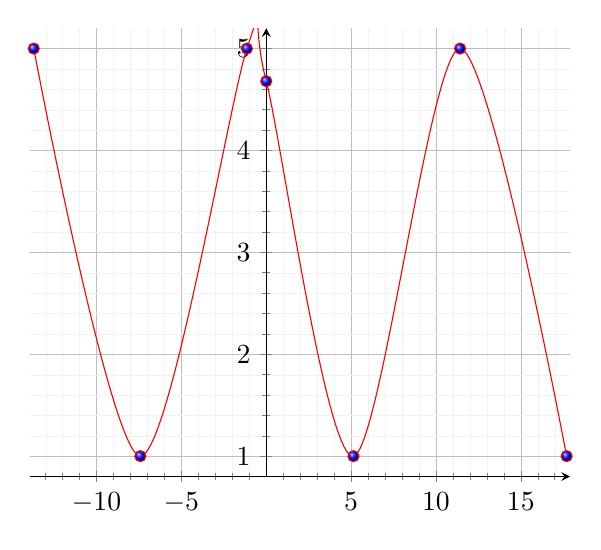
\begin{tikzpicture}
  \begin{axis}%
    [grid=both,
     minor tick num=4,
     grid style={line width=.1pt, draw=gray!10},
     major grid style={line width=.2pt,draw=gray!50},
     axis lines=middle,
     enlargelimits={abs=0.2}
    ]
    \addplot [domain=-13.70:17.7,samples=100,smooth,red,mark=ball]
    % dashed option draws the dashed curve. You can also use dotted, dashdotted, dashdotdotted.  
      coordinates { (-13.70,5) (-7.42,1) (-1.14,5) (0,4.68) (5.14,1) (11.42,5) (17.7,1)};   
  \end{axis}
\end{tikzpicture}
\end{center}
\vspace{5mm}

For the sine function, I made sure that the d was more than 0 so that it couldn't touch the x-axis to fit the A constraint. For the B constraint, I made sure that a was negative so that it would have a positive y-intercept. This would also fit the D constraint because it is a negative value. Then to fit F, I just made sure C was not 0, so I put it as 1.

\vspace{30mm} %5mm vertical space
\hfill \break
Function 2
\hfill \break
Satisfies: C, E, G, H
\begin{displaymath}
    y=-4\cos(0.5x+1)+2
\end{displaymath}

\vspace{5mm}
\begin{center}
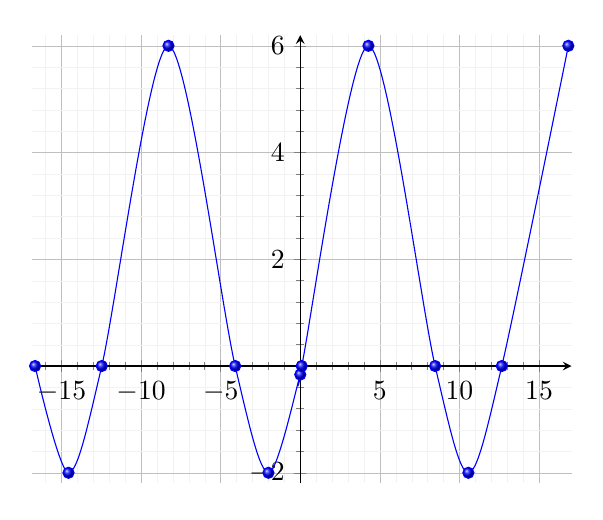
\begin{tikzpicture}
  \begin{axis}%
    [grid=both,
     minor tick num=4,
     grid style={line width=.1pt, draw=gray!10},
     major grid style={line width=.2pt,draw=gray!50},
     axis lines=middle,
     enlargelimits={abs=0.2}
    ]
    \addplot [domain=-13.70:17.7,samples=100,smooth,blue,mark=ball]
    % dashed option draws the dashed curve. You can also use dotted, dashdotted, dashdotdotted.  
      coordinates { (-16.66,0) (-14.56,-2) (-12.47,0) (-8.28,6) (-4.09,0) (-2,-2) (0,-0.16) (0.09,0) (4.28,6) (8.47,0) (10.56,-2) (12.66,0) (16.84, 6)};   
  \end{axis}
\end{tikzpicture}
\end{center}
\vspace{5mm}

For the cosine function, I made sure that the amplitude was greater than the vertical displacement by making d 2. The amplitude is the mid-line, and so 2 is a smaller number than the mid-line. I then ensured that between the points (0, 4), it has exactly one zero. This was where points b and c came in. B made the function skinnier or wider, while g shifted it left or right, and this helped me position it in a place where it would be able to have exactly one zero between the points (0,4). For the period, when you find the period, the formula is 2$\pi$/b, and so I made sure b is a fraction. I then divided 2$\pi$ by whatever b was, and it turned out to be a number that was bigger than 2$\pi$. Lastly, I made sure that the function's range included the negative and positive values. This was where point a came in where it made it longer or shorter, and d was able to move it up and down.

\vfill
\hfill \break
\textbf{Desmos Graphs for better reference}
\hfill \break
\url{https://www.desmos.com/calculator/cyqxvqyxbs}

\end{document}
